\documentclass[tikz]{standalone}

\begin{document}

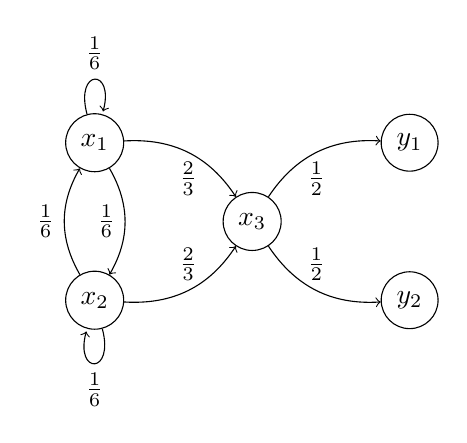
\begin{tikzpicture}
    \node [circle , draw ] (zero) at (0,1) {$x_1$};
    \node [circle , draw ] (one) at (0,-1) {$x_2$};
    \node [circle , draw ] (two) at (2,0) {$x_3$};
    \node [circle , draw ] (three) at (4,1) {$y_1$};
    \node [circle , draw ] (four) at (4,-1) {$y_2$};
    \path[->] (zero) edge [loop above] node {$\frac{1}{6}$} (zero);
    \path[->] (one) edge [loop below] node {$\frac{1}{6}$} (one);
    \path[->] (zero) edge [bend left] node [left] {$\frac{1}{6}$} (one);
    \path[->] (one) edge [bend left] node [left] {$\frac{1}{6}$} (zero);
    \path[->] (zero) edge [bend left] node [below] {$\frac{2}{3}$} (two);
    \path[->] (one) edge [bend right] node [above] {$\frac{2}{3}$} (two);
    \path[->] (two) edge [bend left] node [below] {$\frac{1}{2}$} (three);
    \path[->] (two) edge [bend right] node [above] {$\frac{1}{2}$} (four);
\end{tikzpicture}
\end{document}
